\subsection{习题}\label{sec:2.5}
\setcounter{exercise}{0}
\begin{exercise}\label{exercise:2.1}
在下列各情形中求 $Y$ 的概率密度函数，并证明其积分为 $1$.
\begin{enumerate}
\item[(a)] $Y=X^3$，$f_X(x)=42x^5(1-x)$，$0<x<1$.
\item[(b)] $Y=4X+3$，$f_X(x)=7e^{-7x}$，$0<x<\infty$.
\item[(c)] $Y=X^2$，$f_X(x)=30x^2(1-x)^2$，$0<x<1$.
\end{enumerate}
（见计算机代数附录中的\autoref{ex:12.6.2}.）
\end{exercise}
\begin{exercise}\label{exercise:2.2}
在下列各情形中求 $Y$ 的概率密度函数.
\begin{enumerate}
\item[(a)] $Y=X^2$，$f_X(x)=1$，$0<x<1$.
\item[(b)] $Y=-\log X$，$X$ 的密度为
$$f_X(x)=\frac{(n+m+1)!}{n!m!}x^n(1-x)^m,\qquad0<x<1,\quad m,n\text{ 为正整数}.$$
\item[(c)] $Y=e^X$，$X$ 的密度为
$$f_X(x)=\frac1{\sigma^2}xe^{-(x/\sigma)^2/2},\qquad0<x<\infty,\quad\sigma^2\text{ 为正常数}.$$
\end{enumerate}
\end{exercise}
\begin{exercise}\label{exercise:2.3}
设 $X$ 具有几何概率质量函数 $f_X(x)=\frac13(\frac23)^x$，$x=0,1,2,\ldots$. 求 $Y=X/(X+1)$ 的概率分布. 注意，这里 $X$ 和 $Y$ 都是离散随机变量. 要确定 $Y$ 的概率分布，应给出它的概率质量函数.
\end{exercise}
\begin{exercise}\label{exercise:2.4}
设 $\lambda$ 为固定正常数，定义函数 $f(x)$：当 $x\ge0$ 时，$f(x)=\frac12\lambda e^{-\lambda x}$；当 $x<0$ 时，$f(x)=\frac12\lambda e^{\lambda x}$.
\begin{enumerate}
\item[(a)] 验证 $f(x)$ 是概率密度函数.
\item[(b)] 若随机变量 $X$ 的密度为 $f(x)$，求所有 $t$ 对应的 $P(X<t)$. 算出所有积分.
\item[(c)] 求所有 $t$ 对应的 $P(|X|<t)$. 算出所有积分.
\end{enumerate}
\end{exercise}
\sourcepageanchor{94}
\begin{exercise}\label{exercise:2.5}
用\autoref{thm:2.1.8}求\autoref{ex:2.1.2}中 $Y$ 的概率密度函数. 证明，对\eqref{eq:2.1.6}给出的累积分布函数求导会得到相同答案.
\end{exercise}
\begin{exercise}\label{exercise:2.6}
在下列各情形中求 $Y$ 的概率密度函数，并证明其积分为 $1$.
\begin{enumerate}
\item[(a)] $f_X(x)=\frac12e^{-|x|}$，$-\infty<x<\infty$；$Y=|X|^3$.
\item[(b)] $f_X(x)=\frac38(x+1)^2$，$-1<x<1$；$Y=1-X^2$.
\item[(c)] $f_X(x)=\frac38(x+1)^2$，$-1<x<1$；当 $X\le0$ 时 $Y=1-X^2$，当 $X>0$ 时 $Y=1-X$.
\end{enumerate}
\end{exercise}
\begin{exercise}\label{exercise:2.7}
设 $X$ 的概率密度函数为 $f_X(x)=\frac29(x+1)$，$-1\le x\le2$.
\begin{enumerate}
\item[(a)]\phantomsection\label{itm:exercise:2.7:a} 求 $Y=X^2$ 的概率密度函数. 注意，\autoref{thm:2.1.8}不能直接用于本题.
\item[(b)] 证明，当集合 $A_0,A_1,\ldots,A_k$ 包含 $\mathscr X$ 时，\autoref{thm:2.1.8}仍然成立；并取 $A_0=\varnothing$、$A_1=(-2,0)$、$A_2=(0,2)$，用这一推广解答 \hyperref[itm:exercise:2.7:a]{(a)}.
\end{enumerate}
\end{exercise}
\begin{exercise}\label{exercise:2.8}
对下列各情形，证明给定函数是累积分布函数，并求 $F_X^{-1}(y)$.
\begin{enumerate}
\item[(a)] $F_X(x)=\begin{cases}0,&x<0,\\1-e^{-x},&x\ge0.\end{cases}$
\item[(b)] $F_X(x)=\begin{cases}e^x/2,&x<0,\\1/2,&0\le x<1,\\1-(e^{1-x}/2),&1\le x.\end{cases}$
\item[(c)]\phantomsection\label{itm:exercise:2.8:c} $F_X(x)=\begin{cases}e^x/4,&x<0,\\1-(e^{-x}/4),&x\ge0.\end{cases}$
\end{enumerate}
注意，\hyperref[itm:exercise:2.8:c]{(c)} 中 $F_X(x)$ 不连续，但\eqref{eq:2.1.13}仍然是 $F_X^{-1}(y)$ 的合适定义.
\end{exercise}
\begin{exercise}\label{exercise:2.9}
若随机变量 $X$ 的概率密度函数为
$$f(x)=\begin{cases}\dfrac{x-1}2,&1<x<3,\\0,&\text{其他},\end{cases}$$
求一个单调函数 $u(x)$，使随机变量 $Y=u(X)$ 具有 $\operatorname{uniform}(0,1)$ 分布.
\end{exercise}
\begin{exercise}\label{exercise:2.10}\index{SI0849@离散}\index{SI0988@较大}
\autoref{thm:2.1.10}证明了概率积分变换，把均匀累积分布函数与任意连续累积分布函数联系起来. 本题研究离散随机变量与均匀随机变量之间的关系. 设 $X$ 是累积分布函数为 $F_X(x)$ 的离散随机变量，定义 $Y=F_X(X)$.
\begin{enumerate}
\item[(a)] 证明，$Y$ 在随机意义下大于 $\operatorname{uniform}(0,1)$；即若 $U\sim\operatorname{uniform}(0,1)$，则
$$\begin{aligned}
P(Y>y)&\ge P(U>y)=1-y,&&\text{对所有 $0<y<1$},\\
P(Y>y)&>P(U>y)=1-y,&&\text{对某个 $0<y<1$}.
\end{aligned}$$
（回顾，\autoref{exercise:1.49}定义了“在随机意义下大于”.）
\item[(b)] 等价地，证明 $Y$ 的累积分布函数满足：对所有 $0<y<1$，$F_Y(y)\le y$，并且对某个 $0<y<1$，$F_Y(y)<y$. （提示：设 $x_0$ 为 $F_X$ 的一个跳跃点，定义 $y_0=F_X(x_0)$. 证明 $P(Y\le y_0)=y_0$. 然后考虑 $y=y_0+\varepsilon$，建立所需不等式. 画累积分布函数的图会有帮助.）
\end{enumerate}
\end{exercise}
\begin{exercise}\label{exercise:2.11}
设 $X$ 具有标准正态密度 $f_X(x)=(1/\sqrt{2\pi})e^{-x^2/2}$.
\begin{enumerate}
\item[(a)] 直接求 $\mathrm EX^2$；然后利用\autoref{ex:2.1.7}中 $Y=X^2$ 的密度，计算 $\mathrm EY$，再次求出结果.
\item[(b)] 求 $Y=|X|$ 的概率密度函数，并求它的均值和方差.
\end{enumerate}
\end{exercise}
\begin{exercise}\label{exercise:2.12}\index{SI0277@生成}
可以按下列方式构造随机直角三角形. 设 $X$ 是在 $(0,\pi/2)$ 上均匀分布的随机角. 对每个 $X$，如下图构造三角形，其中 $Y$ 为该随机三角形的高. 对固定常数 $d$，求 $Y$ 的分布和 $\mathrm EY$.
\sourcepageanchor{95}
\begin{center}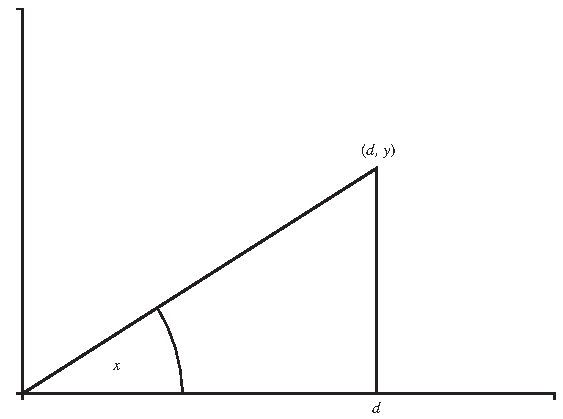
\includegraphics[width=.7\textwidth]{assets/chapter2/exercise2-12.pdf}\end{center}
\end{exercise}
\begin{exercise}\label{exercise:2.13}
考虑一列相互独立的抛硬币试验，每次正面朝上的概率为 $p$. 定义随机变量 $X$ 为从第一次试验开始的游程（正面或反面连续出现）的长度. （例如，观察到 TTTH 或 HHHT 时，都有 $X=3$.）求 $X$ 的分布及 $\mathrm EX$.
\end{exercise}
\needspace{5\baselineskip}
\begin{exercise}\label{exercise:2.14}\index{SI0536@连续}\index{SI0537@离散}\leavevmode
\begin{enumerate}
\item[(a)]\phantomsection\label{itm:exercise:2.14:a} 设 $X$ 是连续的非负随机变量［当 $x<0$ 时，$f(x)=0$］. 证明
$$\mathrm EX=\int_0^\infty[1-F_X(x)]\,dx,$$
其中 $F_X(x)$ 为 $X$ 的累积分布函数.
\item[(b)] 设 $X$ 是取值范围为非负整数的离散随机变量. 证明
$$\mathrm EX=\sum_{k=0}^\infty(1-F_X(k)),$$
其中 $F_X(k)=P(X\le k)$. 将此与 \hyperref[itm:exercise:2.14:a]{(a)} 比较.
\end{enumerate}
\end{exercise}
\begin{exercise}\label{exercise:2.15}\index{SI0431@极大值与极小值的}
\hyperref[bib:source30]{Betteley (1977)} 给出了一个有趣的期望加法法则. 设 $X,Y$ 为任意两个随机变量，定义
$$X\wedge Y=\min(X,Y),\qquad X\vee Y=\max(X,Y).$$
仿照概率法则 $P(A\cup B)=P(A)+P(B)-P(A\cap B)$，证明
$$\mathrm E(X\vee Y)=\mathrm EX+\mathrm EY-\mathrm E(X\wedge Y).$$
（提示：证明 $X+Y=(X\vee Y)+(X\wedge Y)$.）
\end{exercise}
\begin{exercise}\label{exercise:2.16}
用\autoref{exercise:2.14}的结果求某类电话通话的平均时长. 假设一次通话的时长 $T$ 可用下列概率关系描述：$P(T>t)=ae^{-\lambda t}+(1-a)e^{-\mu t}$，其中 $a,\lambda,\mu$ 为常数，$0<a<1$，$\lambda>0$，$\mu>0$.
\end{exercise}
\begin{exercise}\label{exercise:2.17}\index{SI0684@中位数}
分布的中位数（median）是满足 $P(X\le m)\ge\frac12$ 且 $P(X\ge m)\ge\frac12$ 的数 $m$. （若 $X$ 连续，则 $m$ 满足 $\int_{-\infty}^m f(x)\,dx=\int_m^\infty f(x)\,dx=\frac12$.）求下列分布的中位数.
\begin{enumerate}
\item[(a)] $f(x)=3x^2$，$0<x<1$.
\item[(b)] $f(x)=1/[\pi(1+x^2)]$，$-\infty<x<\infty$.
\end{enumerate}
\end{exercise}
\begin{exercise}\label{exercise:2.18}\index{SI0685@最小化性质}
证明，如果 $X$ 是连续随机变量，则
$$\min_a\mathrm E|X-a|=\mathrm E|X-m|,$$
其中 $m$ 为 $X$ 的中位数（见\autoref{exercise:2.17}）.
\end{exercise}
\sourcepageanchor{96}
\begin{exercise}\label{exercise:2.19}
通过对积分求导，证明
$$\frac d{da}\mathrm E(X-a)^2=0\ \Longleftrightarrow\ \mathrm EX=a.$$
用微积分验证 $a=\mathrm EX$ 确实给出最小值. 列出关于 $F_X$ 和 $f_X$ 所需的假设.
\end{exercise}
\begin{exercise}\label{exercise:2.20}
一对夫妇决定不断生育，直到生出一个女儿为止. 这对夫妇的子女数的期望是多少？（提示：见\autoref{ex:1.5.4}.）
\end{exercise}
\begin{exercise}\label{exercise:2.21}
证明期望的“双向”法则\eqref{eq:2.2.5}，即 $\mathrm Eg(X)=\mathrm EY$，其中 $Y=g(X)$. 假定 $g(x)$ 为单调函数.
\end{exercise}
\begin{exercise}\label{exercise:2.22}
设 $X$ 的概率密度函数为
$$f(x)=\frac4{\beta^3\sqrt\pi}x^2e^{-x^2/\beta^2},\qquad0<x<\infty,\quad\beta>0.$$
\begin{enumerate}
\item[(a)] 验证 $f(x)$ 是概率密度函数.
\item[(b)] 求 $\mathrm EX$ 和 $\operatorname{Var}X$.
\end{enumerate}
\end{exercise}
\begin{exercise}\label{exercise:2.23}
设 $X$ 的概率密度函数为
$$f(x)=\frac12(1+x),\qquad-1<x<1.$$
\begin{enumerate}
\item[(a)] 求 $Y=X^2$ 的概率密度函数.
\item[(b)] 求 $\mathrm EY$ 和 $\operatorname{Var}Y$.
\end{enumerate}
\end{exercise}
\begin{exercise}\label{exercise:2.24}
对下列每个概率分布，计算 $\mathrm EX$ 和 $\operatorname{Var}X$.
\begin{enumerate}
\item[(a)] $f_X(x)=ax^{a-1}$，$0<x<1$，$a>0$.
\item[(b)] $f_X(x)=1/n$，$x=1,2,\ldots,n$，$n>0$ 为整数.
\item[(c)] $f_X(x)=\frac32(x-1)^2$，$0<x<2$.
\end{enumerate}
\end{exercise}
\begin{exercise}\label{exercise:2.25}\index{SI0832@偶}
设随机变量 $X$ 的概率密度函数 $f_X(x)$ 为偶函数. （若对每个 $x$，都有 $f_X(x)=f_X(-x)$，则 $f_X(x)$ 称为偶函数.）证明
\begin{enumerate}
\item[(a)] $X$ 与 $-X$ 同分布.
\item[(b)] $M_X(t)$ 关于零对称.
\end{enumerate}
\end{exercise}
\begin{exercise}\label{exercise:2.26}\index{SI0840@对称}
设 $f(x)$ 为概率密度函数，$a$ 为一个数，使得对所有 $\varepsilon>0$ 都有 $f(a+\varepsilon)=f(a-\varepsilon)$. 称这样的密度关于点 $a$ 对称（symmetric）.
\begin{enumerate}
\item[(a)] 举出三个对称密度的例子.
\item[(b)] 证明，如果 $X\sim f(x)$ 且该密度对称，则 $X$ 的中位数（见\autoref{exercise:2.17}）是 $a$.
\item[(c)] 证明，如果 $X\sim f(x)$ 且该密度对称，$\mathrm EX$ 存在，则 $\mathrm EX=a$.
\item[(d)]\phantomsection\label{itm:exercise:2.26:d} 证明，$f(x)=e^{-x}$，$x\ge0$，不是对称密度.
\item[(e)] 证明，对 \hyperref[itm:exercise:2.26:d]{(d)} 中的密度，中位数小于均值.
\end{enumerate}
\end{exercise}
\begin{exercise}\label{exercise:2.27}\index{SI0842@单峰}
设 $f(x)$ 为概率密度函数，$a$ 为一个数，使得当 $a\ge x\ge y$ 时，$f(a)\ge f(x)\ge f(y)$；当 $a\le x\le y$ 时，也有 $f(a)\ge f(x)\ge f(y)$. 称这样的密度为单峰（unimodal）密度，$a$ 为一个众数（mode）.
\begin{enumerate}
\item[(a)] 举出一个众数唯一的单峰密度.
\item[(b)] 举出一个众数不唯一的单峰密度.
\item[(c)] 证明，如果 $f(x)$ 既对称（见\autoref{exercise:2.26}）又单峰，则其对称中心是一个众数.
\item[(d)] 考虑密度 $f(x)=e^{-x}$，$x\ge0$. 证明该密度单峰. 它的众数是什么？
\end{enumerate}
\end{exercise}
\begin{exercise}\label{exercise:2.28}\index{SI0599@峰度}\index{SI0978@偏度}
令 $\mu_n$ 表示随机变量 $X$ 的 $n$ 阶中心矩. 除均值与方差外，另外两个值得关注的量是
$$\alpha_3=\frac{\mu_3}{(\mu_2)^{3/2}},\qquad\alpha_4=\frac{\mu_4}{\mu_2^2}.$$
$\alpha_3$ 称为偏度（skewness），$\alpha_4$ 称为峰度（kurtosis）. 偏度衡量密度的不对称性（见\autoref{exercise:2.26}）. 峰度虽然更难解释，但它衡量密度的尖峭或平坦程度.
\begin{enumerate}
\item[(a)] 证明，如果一个密度关于点 $a$ 对称，则 $\alpha_3=0$.
\item[(b)] 计算 $f(x)=e^{-x}$，$x\ge0$ 的 $\alpha_3$；这是一个右偏（skewed to the right）的密度.
\sourcepageanchor{97}
\item[(c)] 对下列每个密度计算 $\alpha_4$，并评论其尖峭程度.
$$\begin{aligned}
f(x)&=\frac1{\sqrt{2\pi}}e^{-x^2/2},&-\infty<x<\infty,\\
f(x)&=\frac12,&-1<x<1,\\
f(x)&=\frac12e^{-|x|},&-\infty<x<\infty.
\end{aligned}$$
\end{enumerate}
\hyperref[bib:source268]{Ruppert (1987)} 用影响函数（influence function，\autoref{sec:10.6.4}）进一步研究峰度的含义，\hyperref[bib:source152]{Groeneveld (1991)} 用它研究偏度；关于 $\alpha_4$ 的解释，还可参见 \hyperref[bib:source6]{Balanda and MacGillivray (1988)}.
\end{exercise}
\begin{exercise}\label{exercise:2.29}
计算离散分布的矩时，使用阶乘矩（factorial moments）往往更容易（见\hyperref[sec:2.6.2]{杂录~2.6.2}）.
\begin{enumerate}
\item[(a)]\phantomsection\label{itm:exercise:2.29:a} 计算二项分布和泊松分布的阶乘矩 $\mathrm E[X(X-1)]$.
\item[(b)] 用 \hyperref[itm:exercise:2.29:a]{(a)} 的结果计算二项分布和泊松分布的方差.
\item[(c)] 一个特别难处理的离散分布是贝塔二项分布（beta-binomial），其概率质量函数为
$$P(y=y)=a(y+a)\frac{\binom ny\binom{a+b-1}a}{\binom{n+a+b-1}{y+a}},$$
其中 $n,a,b$ 为整数，$y=0,1,2,\ldots,n$. 用阶乘矩计算贝塔二项分布的方差. （这一计算的另一种方法见\autoref{exercise:4.34}.）\footnote{译注：原文左端写作 $P(y=y)$，随机变量通常应大写为 $Y$. 原式前因子 $a(y+a)$ 也有疑误：例如 $n=a=b=1$ 时，两项质量为 $1/2$ 与 $2$，和不为 $1$. 将该因子改为 $a/(y+a)$，才得到通常的贝塔二项质量函数；此外通常要求 $a,b>0$. 此处保留原式与原假设.}
\end{enumerate}
\end{exercise}
\begin{exercise}\label{exercise:2.30}
求下列分布的矩母函数.
\begin{enumerate}
\item[(a)] $f(x)=1/c$，$0<x<c$.
\item[(b)] $f(x)=2x/c^2$，$0<x<c$.
\item[(c)] $f(x)=\frac1{2\beta}e^{-|x-\alpha|/\beta}$，$-\infty<x<\infty$，$-\infty<\alpha<\infty$，$\beta>0$.
\item[(d)] $P(X=x)=\binom{r+x-1}x p^r(1-p)^x$，$x=0,1,\ldots$，$0<p<1$，$r>0$ 为整数.
\end{enumerate}
\end{exercise}
\begin{exercise}\label{exercise:2.31}
是否存在一个分布，其矩母函数为 $M_X(t)=t/(1-t)$，$|t|<1$？如果存在，求出它；如果不存在，证明之.
\end{exercise}
\begin{exercise}\label{exercise:2.32}
设 $M_X(t)$ 为 $X$ 的矩母函数，定义 $S(t)=\log(M_X(t))$. 证明
$$\left.\frac d{dt}S(t)\right|_{t=0}=\mathrm EX,\qquad
\left.\frac{d^2}{dt^2}S(t)\right|_{t=0}=\operatorname{Var}X.$$
\end{exercise}
\begin{exercise}\label{exercise:2.33}
对下列各情形，验证给出的矩母函数表达式，并利用它计算 $\mathrm EX$ 和 $\operatorname{Var}X$.
\begin{enumerate}
\item[(a)] $P(X=x)=e^{-\lambda}\lambda^x/x!$，$M_X(t)=e^{\lambda(e^t-1)}$，$x=0,1,\ldots$；$\lambda>0$.
\item[(b)] $P(X=x)=p(1-p)^x$，$M_X(t)=p/[1-(1-p)e^t]$，$x=0,1,\ldots$；$0<p<1$.
\item[(c)] $f_X(x)=e^{-(x-\mu)^2/(2\sigma^2)}/(\sqrt{2\pi}\sigma)$，$M_X(t)=e^{\mu t+\sigma^2t^2/2}$，$-\infty<x<\infty$；$-\infty<\mu<\infty$，$\sigma>0$.
\end{enumerate}
\end{exercise}
\begin{exercise}\label{exercise:2.34}
有限个矩不能唯一确定一个分布，\hyperref[bib:source258]{Romano and Siegel (1986)} 中的这个例子说明了这一点. 设 $X$ 具有正态分布，即密度为
$$f_X(x)=\frac1{\sqrt{2\pi}}e^{-x^2/2},\qquad-\infty<x<\infty.$$
定义离散随机变量 $Y$：
$$P(Y=\sqrt3)=P(Y=-\sqrt3)=\frac16,\qquad P(Y=0)=\frac23.$$
证明
$$\mathrm EX^r=\mathrm EY^r,\qquad r=1,2,3,4,5.$$
（\hyperref[bib:source258]{Romano and Siegel (1986)} 指出，对任意有限的 $n$，都存在一个离散的、从而非正态的随机变量，其前 $n$ 阶矩与 $X$ 的对应矩相同.）
\end{exercise}
\sourcepageanchor{98}
\begin{exercise}\label{exercise:2.35}\index{SI0698@非唯一性}
补全\autoref{ex:2.3.10}中的细节.
\begin{enumerate}
\item[(a)] 证明，若 $X_1\sim f_1(x)$，则
$$\mathrm EX_1^r=e^{r^2/2},\qquad r=0,1,\ldots.$$
所以 $f_1(x)$ 的所有阶矩都存在，并且全都有限.
\item[(b)] 证明，对所有正整数 $r$，
$$\int_0^\infty x^rf_1(x)\sin(2\pi\log x)\,dx=0,$$
因而对所有 $r$，$\mathrm EX_1^r=\mathrm EX_2^r$. （\hyperref[bib:source258]{Romano and Siegel (1986)} 讨论了这个例子的极端版本，即一整类不同的密度具有相同的各阶矩. 此外，\hyperref[bib:source16]{Berg (1988)} 表明，正态分布的较简单变换，例如 $X^3$，也会出现这种矩的现象.）
\end{enumerate}
\end{exercise}
\begin{exercise}\label{exercise:2.36}\index{SI0333@矩母函数}
\autoref{ex:2.3.10}所依据的对数正态分布具有一个有趣性质. 若密度为
$$f(x)=\frac1{\sqrt{2\pi}x}e^{-(\log x)^2/2},\qquad0\le x<\infty,$$
则\autoref{exercise:2.35}表明所有阶矩都存在且有限. 然而，这个分布没有矩母函数，即
$$M_X(t)=\int_0^\infty\frac{e^{tx}}{\sqrt{2\pi}x}e^{-(\log x)^2/2}\,dx$$
不存在. 证明之.
\end{exercise}
\begin{exercise}\label{exercise:2.37}
参照\hyperref[sec:2.6.3]{杂录~2.6.3}所述的情形：
\begin{enumerate}
\item[(a)] 画出密度 $f_1$ 和 $f_2$，说明它们的差异.
\item[(b)] 画出累积量母函数 $K_1$ 和 $K_2$，说明它们的相似性.
\item[(c)] 计算密度 $f_1$ 和 $f_2$ 的矩母函数. 它们相似还是不同？
\item[(d)] 密度 $f_1$ 和 $f_2$ 与\autoref{ex:2.3.10}中的密度有什么关系？
\end{enumerate}
\end{exercise}
\begin{exercise}\label{exercise:2.38}\index{SI0283@与负二项的关系}\index{SI0354@与卡方的关系}
设 $X$ 具有负二项分布（negative binomial distribution），概率质量函数为
$$f(x)=\binom{r+x-1}x p^r(1-p)^x,\qquad x=0,1,2,\ldots,$$
其中 $0<p<1$，$r>0$ 为整数.
\begin{enumerate}
\item[(a)] 计算 $X$ 的矩母函数.
\item[(b)] 定义新随机变量 $Y=2pX$. 证明，当 $p\downarrow0$ 时，$Y$ 的矩母函数收敛到自由度为 $2r$ 的卡方随机变量的矩母函数，即证明
$$\lim_{p\to0}M_Y(t)=\left(\frac1{1-2t}\right)^r,\qquad |t|<\frac12.$$
\end{enumerate}
\end{exercise}
\begin{exercise}\label{exercise:2.39}
对下列各情形计算所示导数，并说明所有运算的合理性.
\begin{enumerate}
\item[(a)] $\displaystyle\frac d{dx}\int_0^x e^{-\lambda t}\,dt$.
\item[(b)] $\displaystyle\frac d{d\lambda}\int_0^\infty e^{-\lambda t}\,dt$.
\item[(c)] $\displaystyle\frac d{dt}\int_t^1\frac1{x^2}\,dx$.
\item[(d)] $\displaystyle\frac d{dt}\int_1^\infty\frac1{(x-t)^2}\,dx$.
\end{enumerate}
\end{exercise}
\begin{exercise}\label{exercise:2.40}\index{SI0257@与二项的关系}\index{SI0268@与贝塔的关系}
证明
$$\sum_{k=0}^x\binom nk p^k(1-p)^{n-k}
=(n-x)\binom nx\int_0^{1-p}t^{n-x-1}(1-t)^x\,dt.$$
（提示：分部积分，或两边对 $p$ 求导.）
\end{exercise}
